\documentclass{article}

% ------ TEMPLATE ------ %

% ---------------------- %

% ------ PACKAGES ------ %

\usepackage{charter}
\usepackage{geometry}
\usepackage{amsmath}
\usepackage{amssymb}
\usepackage{float}
\usepackage{graphicx}
\usepackage{tabularx}
\usepackage{array}
\usepackage{subcaption}
\usepackage{enumitem}
\usepackage{titlesec}
\usepackage{hyperref}
\usepackage{xcolor}
\usepackage{pifont}
\usepackage{fancyvrb}
\usepackage{listings}
\usepackage{multirow}
\usepackage{ulem}

% ---------------------- %

% ------ GENERALS ------ %

\setlist[itemize]{label=\scriptsize\textbullet}
\setlist[itemize]{noitemsep, topsep=1pt}
\setlist[enumerate]{noitemsep, topsep=1pt}

\titleformat{\chapter}[hang]
{\normalfont\huge\bfseries}{\thechapter}{1em}{}
\titleformat{\subsubsection}{\large\bfseries}{\thesubsubsection}{1em}{}

% ---------------------- %

% ------- COLORS ------- %

\hypersetup{
    colorlinks=true,
    linkcolor=blue!50!black,
    urlcolor=blue,
    citecolor=blue,
    pdfborder={0 0 0}
}

% ---------------------- %

% ------ COMMANDS ------ %

\newcommand{\vmark}{\textcolor{teal}{\ding{51}}}
\newcommand{\xmark}{\textcolor{red!70!black}{\ding{55}}}
\newcommand{\newpar}[0]{\vspace{2mm}\noindent}
\newcommand{\htitle}[1]{\newpar\textbf{#1 -}}
\newcommand{\ititle}[1]{\newpar\hspace{1em}\textbf{#1}}
\newcommand{\hyperlabel}[1]{\hypertarget{#1}\phantomsection\label{#1}}
\newcommand{\hyperitem}[2]{\item \hyperlink{#1}{#2}\leaders\hbox to 0.8em{\hss.\hss}\hfill\hbox to 1.8em{\hss\pageref{#1}}}
\newcommand{\stdtilde}[0]{\raise.17ex\hbox{$\scriptstyle\sim$}}
\newcommand{\xor}[0]{\char`\^}
\newcommand{\saveformula}[2]{\newbox{#1}\savebox{#1}{#2}}
\newcommand{\useformula}[1]{\usebox{#1}}

% ---------------------- %

\begin{document}

% -------- HEAD -------- %

\pagenumbering{gobble}

\begin{center}

    \fontsize{20pt}{30pt}\selectfont
    Well MEing

    \vspace{2cm}

    \fontsize{25pt}{45pt}\selectfont
    \textbf{Practical Development Overview}

    \vfill

    \fontsize{12pt}{18pt}\selectfont
    Matteo Bettiati \\
    Lorenzo Bianchi \\
    Alessio Caggiano \\
    Francesco Ostidich \\
    Denis Sanduleanu \\

    \vspace{1cm}

    \today \\
    \vspace{12pt}
    Version: 1.0
    \normalsize

\end{center}

\newpage
\pagenumbering{arabic}
\tableofcontents
\newpage

% ---------------------- %

% -------- BODY -------- %

\section{Introduction}

\subsection{Purpose of the document}

This document outlines the practical development overview for Well MEing, a highly customizable wellness tracking application.
The goal is to deliver a mobile-first, engaging, and AI-assisted experience that empowers users to track the aspects of well-being that matter most to them, from fitness and nutrition to sleep and stress management.

Built upon the insights gathered in our Product Research Report (PRR), this document presents a comprehensive view of the application's envisioned use cases, technical architecture, and implementation roadmap.
Through thoughtful design and modern development practices, we aim to address user pain points identified during the research by bringing a compelling and effective solution to the market.

\subsection{Definitions}

% TODO
\begin{itemize}
    \item \textbf{Habit/group:} a specific behavior or activity that a user wants to track and improve.
    \item \textbf{Metric:} a quantifiable measure of a habit, such as steps taken, hours slept, or glasses of water consumed.
    \item \textbf{Goal/target/objective:} a specific value or range that a user aims to achieve for a habit or metric, such as "Drink 8 glasses of water per day" or "Sleep 7 hours per night."
    \item \textbf{Assistant:} the AI-driven feature that provides personalized insights and recommendations.
    \item \textbf{Progress/statistics/charts:} visual representations of user data over time, helping users understand their habits and track their progress toward goals.
\end{itemize}

\section{User interaction}

\subsection{Features}

The table below displays the prioritized features that we plan to develop in various scenarios.

\begin{table}[H]
    \centering
    \begin{tabularx}{0.5\textwidth}{c|X}
        \hline
        \textbf{Rank} & \textbf{Feature} \\
        \hline
        1 & Custom habit creation \\
        2 & Minimalistic UI \\
        3 & Quick habit logging  \\
        4 & AI-generated progress reports  \\
        5 & Voice-based interaction  \\
        6 & Targets \\
        7 & Configurable notifications  \\
        8 & Adaptable data visualization \\
        \hline
    \end{tabularx}
\end{table}

\subsection{Scenarios}

This section presents practical use case scenarios that demonstrate how the application will serve its diverse user base in real-life situations.
These scenarios directly resembles the feature list defined in the user research, focussing on the themes and needs that user mentionned the most.

\vspace{5pt}
\begin{enumerate}[label=\textbf{S\arabic* -}]
    \setlength{\itemsep}{5pt}

    \item \textbf{Habit creation, logging and goal setting -}
        Anna wants to track her daily water intake and study hours.
        She opens \textit{Well MEing}, finding herself on the dashboard main page, and by tapping "Create Habit" she can defines two custom habits: "Drink Water" (measured in glasses per day) and "Study Time" (hours per day).
        She selects intuitive input types like sliders and number fields.
        A descriptive button for each habit is now shown on the dashboard.
        By tapping the "Study Time" button, a pop up appears, letting Anna set up a goal ("30 hours a week").
        Each day, she can log her progress with just two taps from the dashboard, from which she can also see her progress towards the goals she set.

    \item \textbf{AI-generated report and custom notifications -}
        Luca uses \textit{Well MEing} to monitor his sleep and stress levels.
        Each week, the app generates a personalized AI-driven report summarizing his trends: "You slept an average of 7 hours/night. Higher stress was detected on days with less than 6 hours of sleep. Try reducing screen time before bed".
        Luca customizes his notifications to receive a reminder at 10 PM for sleep preparation.

    \item \textbf{Check the progress -}
        Sofia has been tracking her daily step count and hydration over the past month.
        She opens \textit{Well MEing} and navigates to the progress section, where she views a bar chart showing her daily step count over time.
        She notices a trend: her step count is higher on weekdays than weekends.
        The hydration graph shows that she consistently meets her target of 8 glasses/day.
        She uses this information to adjust her weekend routine to include more physical activity.

    \item \textbf{Voice-based habit logging and creation -}
        Roberto wants to log his daily activities, but since he is cooking, he opts for the speech-logging option.
        After opening the application, he taps the “Speech Assistant” button and starts speaking, stating that he ran 8 km that day.
        As he is training for a marathon next month, he also asks Well MEing to create a new habit: “Daily Calorie Intake”.
        Once he stops the voice recording, a pop-up appears displaying the commands the AI has recognized based on the speech-to-text processing.
        By tapping the “Accept” button, Roberto confirms the actions, successfully logging his habit and creating the new one.

\end{enumerate}

\section{Architectural design}

\subsection{Deployment view}

This diagram illustrates the deployment architecture of the application, showcasing the various components and their interactions.

\begin{figure}
    \centering
    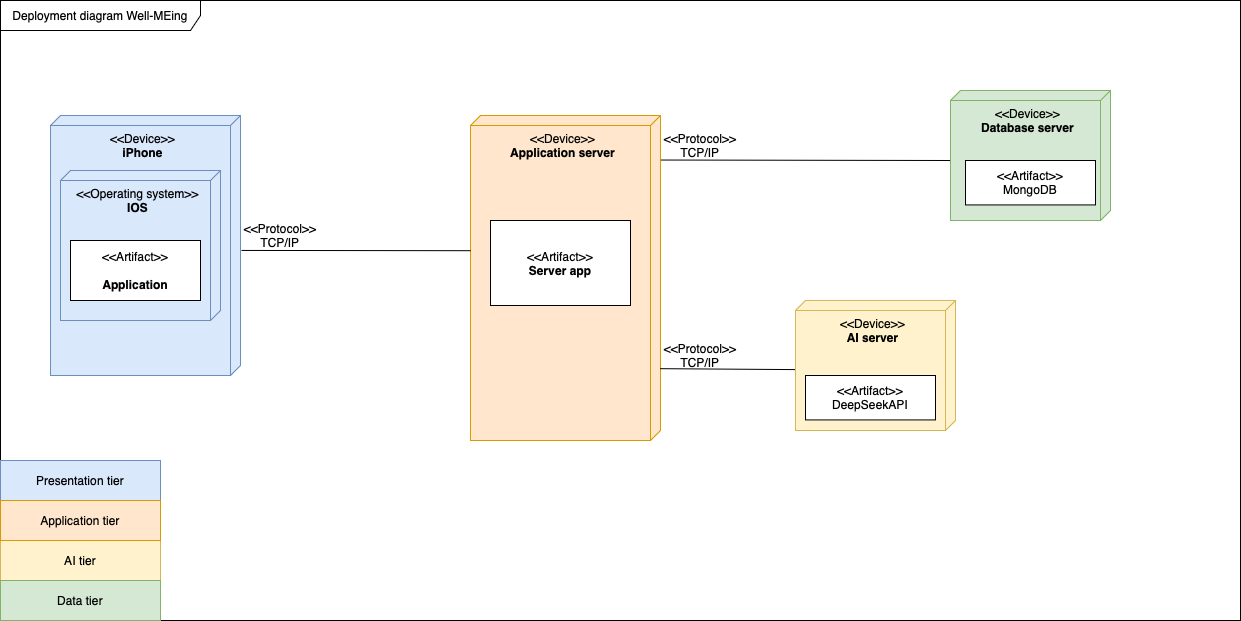
\includegraphics[width=0.8\textwidth]{images/DeploymentView.png}
    \caption{Deployment architecture of the application}
    \label{fig:deployment_diagram}
\end{figure}

\subsection{Components view}

The components view diagram provides a detailed breakdown of the application's architecture, highlighting the key components and their interactions.
\begin{figure}
    \centering
    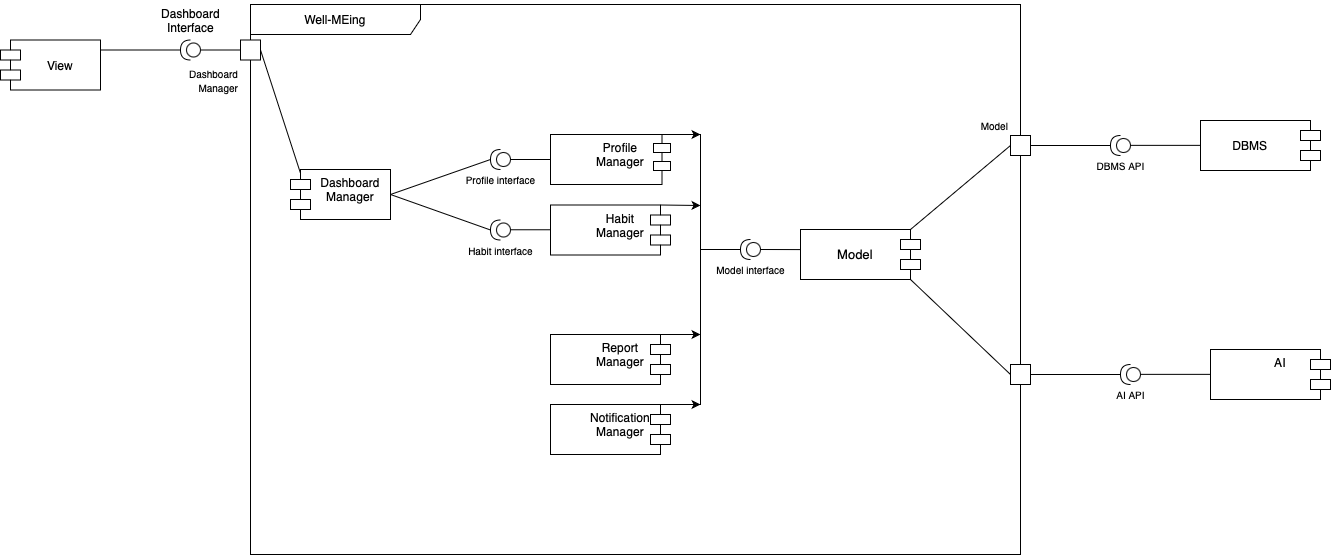
\includegraphics[width=0.8\textwidth]{images/ComponentView.png}
    \caption{Components view of the application}
    \label{fig:components_diagram}
\end{figure}

\subsection{Patterns}

The architectural design of the application is structured according to the principles of various well-known patters (e.g. MVC), ensuring modularity, scalability, and maintainability.
Additionally, the system is organized into a multi-tier architecture, with a dedicated tier for AI services, to support the features requiring and intelligent agent.

\subsubsection{Distributed MVC}

The Model-View-Controller (MVC) design pattern is used to separate the presentation layer from the business logic and data definitions.
In particular, the model contains all the elements representing the data used by the application, the view is the user interface component, and the controller comprehends all the other services and managers.

In this project, the view resides on the client device, the model reflects the database structure (which is a separate application accessed through defined interfaces), and the controller logic is handled by the backend server.
Additionally, the backend relies on another server for AI operations.
As a result, the MVC pattern can be considered “distributed.”

\subsubsection{Clean architecture}

The backend server follows a clean architecture approach, structuring code into distinct layers.

The presentation layer contains controllers that expose API endpoints.
The application layer handles business logic and use cases.
The domain layer defines core entities and interfaces.
The infrastructure layer manages external concerns like database access and communication with an AI backend.

This separation ensures clear boundaries between concerns.

\subsubsection{Four-tier architecture}

The application adopts a four-tier architecture, where each layer has a distinct role while communicating through well-defined interfaces.

The Presentation Tier consists of a native Swift application that serves as the primary interface for users.
The Application Tier represents the backend server, which provides the various services through REST endpoints.
The Data Tier corresponds to the database manager, which lets the backend server access to the main storage.
The AI Service Tier runs independently as a dedicated AI backend, handling mainly natural language processing, exposing its capabilities through APIs.

This four-tier approach promotes maintainability allowing each component to evolve independently while ensuring smooth communication between layers.

\section{Implementation plan}

\subsection{Development roadmap}

We will start development by designing the backend and frontend based on the component view and mockups. 
Both will be built in parallel, with the backend defining the APIs that the frontend will integrate with. Once the core functionality is in place, we will later incorporate AI-related features when they are ready. 
For now, we will focus on identifying potential APIs for the AI layer.

\subsection{Development technologies}

For development, we will use Swift for the frontend to ensure a smooth and responsive user experience. The backend will be built using Java, providing robustness and scalability. 
MongoDB will be our database of choice due to its flexibility in handling dynamic data structures, which aligns well with our application's needs.
\subsection{User interface design}

This section showcases mock-up designs that visualize the user experience and interface of the application.
It also describes the organization of the UI elements across the main app sections, justifying design decisions for content placement and user flow.

The UI is crafted to be minimalist yet engaging, following the principle of simplicity prioritized by users during research.
Each mock-up reflects user-centric design, focusing on accessibility, speed of interaction, and aesthetic appeal, offering a preview of the intuitive and motivating environment we aim to create.

\subsubsection{UI elements organization}

The application will consist of five main pages, structured for an intuitive user experience:

\begin{enumerate}
    \item \textbf{Dashboard:} Provides an overview of tracked habits, progress, and key insights.
    \item \textbf{Calendar:} Displays habit history, upcoming tasks, and scheduling options.
    \item \textbf{Voice Record:} Allows users to log habits or notes using voice input.
    \item \textbf{Report (AI-Based):} Generates insights and analytics based on user habits using AI.
    \item \textbf{Profile Section:} Manages user settings, preferences, and account details.
\end{enumerate}

\subsubsection{Mock-ups}

% image (screenshot) for each main app page

% ---------------------- %

\end{document}